\section{Cifrari di flusso}

\subsection{Definizione}
\begin{frame}
    \frametitle{Cifrari di flusso}
    Un cifrario a flusso è un dispositivo in grado di generare una sequenza di bit dipendente dallo stato iniziale dello stesso con le seguenti proprietà:
    \begin{itemize}
        \item <1-> La periodicità della sequenza di bit deve essere elevata (idealmente infinita)
        \item <2-> Non deve essere possibile ricavare lo stato interno del cifrario data una porzione dello stream di output.
        \item <3-> Il bitstream non deve essere riconoscibile rispetto a un rumore randomico, ovvero la probabilità che ciascun bit possa essere 0 o 1 non deve dipendere dai bit precedenti e deve essere uguale a 0.5
        \item <4-> non devono esserci \textit{``Weak Keys''} o \textit{``Weak States''}
    \end{itemize}
\end{frame}
\note{
    I cifrari di flusso prendono ispirazione da OneTimePad, dove il testo cifrato non è altro che lo xor bit a bit con una chiave.
    In sè OTP è un cifrario perfetto, dato che non permette a un ascoltatore di inferire sulle probabilità che i bit del testo sorgente siano 1 o 0; ciò è valido solo se la chiave è completamente randomica e non viene mai riutilizzata.

    Gli stream cipher sono stati dunque ideati al fine di generare continuamente bit con i quali cifrare la chiave, facendo sì che il bit non dipenda dai precedenti e che esso abbia uguale probabilità di essere in uno stato o nell'altro.

    La convenienza degli stream ciphers sta nel fatto che ritornano lo stesso stream di dati a parità di stato iniziale.
}

\subsection{Struttura}
\begin{frame}
    \frametitle{Struttura}
    Il cifrario di flusso più semplice è un Linear Feedback Shift Register costituito da un solo blocco composto da:
    \begin{itemize}
        \item Un Registro a scorrimento dove, ad ogni iterazione, un bit può essere aggiunto ``in coda'' e il bit più significativo viene scartato.
        \item Una funzione $g(SR)$ che dato lo stato attuale computa il prossimo bit da aggiungere
        \item Una funzione di filtraggio $f(SR)$ che dallo stato del registro computa l'output.
    \end{itemize}

    \begin{figure}
        \centering
        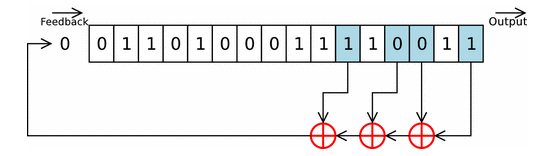
\includegraphics[width=0.4\textwidth]{LFSR.png}
        \caption{Diagramma di un LFSR dove $f(SR)$ è la funzione identità del bit finale}
        \label{fig:lfsr}
    \end{figure}
\end{frame}
\note{
    In questo caso la funzione $g$ è \[g(b_0, b_1, ... b_{16}) = b_{16} \oplus b_{14} \oplus b_{13} \oplus b_{11}\]
    mentre \[f(b_0, b_1, ... b_{16}) = b_{16}\]
}

\begin{frame}
    \frametitle{Struttura}
    È possibile unire più LFSR in una funzione $F(LFSR1, ... LFSRN)$ di filtraggio generale come implementato da A5/1

    \begin{figure}
        \centering
        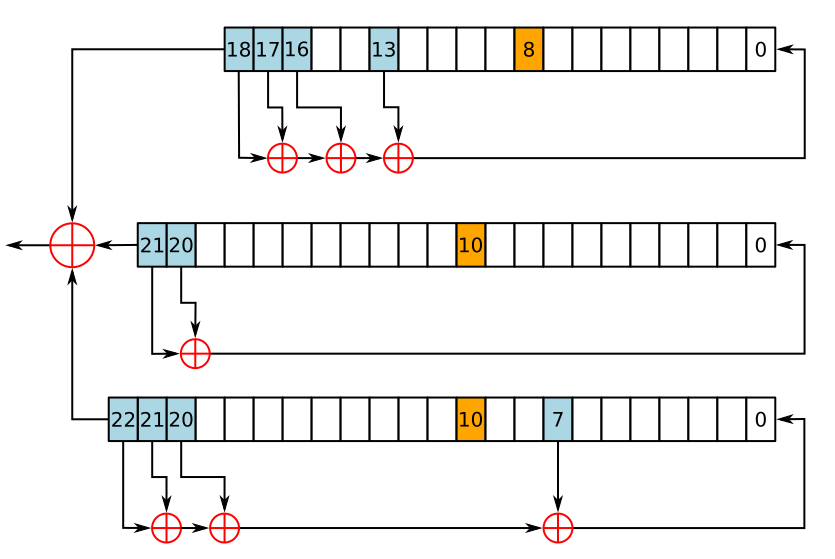
\includegraphics[width=0.4\textwidth]{A51.png}
        \caption{Diagramma di A5/1}
        \label{fig:a51}
    \end{figure}
\end{frame}
\note{
    Per il primo LFSR:
    \[g_1(b_0 ... b_{18}) = b_{18} \oplus b_{17} \oplus b_{16} \oplus b_{13}\]
    \[f_1(b_0 ... b_{18}) = b_{18}\]

    Per il secondo LFSR:
    \[g_2(b_0 ... b_{21}) = b_{21} \oplus b_{20}\]
    \[f_2(b_0 ... b_{21}) = b_{21}\]

    Per il terzo LFSR:
    \[g_3(b_0 ... b_{22}) = b_{22} \oplus b_{21} \oplus b_{20} \oplus b_{7}\]
    \[f_3(b_0 ... b_{22}) = b_{22}\]

    Infine
    \[F(r_1, r_2, r_3) = r_1 \oplus r_2 \oplus r_3\]
}
